\title{Resumen de Analisis Numerico}

\author{Mateo P. Cetti}

\documentclass[10pt]{article}

\usepackage{amsmath}
\usepackage{amsfonts}
\usepackage{graphicx}

\begin{document} 
\maketitle

\section{Equisde}

\paragraph{Equisde_1}

Este texto es muy xd \textbf{doble xd} en algunos casos exhibe características de una \textbf{xd} y en otras de una \textbf{partícula} (onda electromagnetica sinusoidal o rayo de luz)\\
El modelo de cuantización supone que la \textbf{energía} de una onda luminosa está presente en partículas llamadas \textbf{fotones}; por tanto, se dice que la energía está \textbf{cuantizada}. La energía de un fotón es proporcional a la frecuencia de la onda electromagnética. $E = hf \rightarrow h = 6.63 \times 10^{-34} J\cdot s$ donde $h$ es la \textbf{constante de Plank}.\\

\paragraph{Diagramas de rayos para espejos}
Para dibujar el diagrama de un rayo, es necesario conocer la posición del objeto y la localización del foco, así como el centro de curvatura del espejo. Después, dibuje tres rayos principales para localizar la imagen.\\
En el caso de espejos cóncavos, trace los tres rayos principales siguientes
\begin{itemize}
	\item El rayo 1, desde la parte superior del objeto, en paralelo al eje principal, y se refleja a través del foco F
	\item El rayo 2, desde la parte superior del objeto a través del foco (o como si viniera del foco si $p < f$ ) y se refleja paralelo al eje principal.
	\item El rayo 3, desde la parte superior del objeto a través del centro de curvatura C y se refleja de regreso sobre sí mismo.
\end{itemize}
En el caso de los espejos convexos, trace los tres rayos principales siguientes:
\begin{itemize}
	\item El rayo 1 se dibuja desde la parte superior del objeto paralelo al eje principal y se refleja alejándose del foco F.
	\item El rayo 2 El rayo 2, se dibuja desde la parte superior del objeto hacia el foco en la cara posterior del espejo y se refleja paralelo al eje principal.
	\item El rayo 3 se dibuja desde la parte superior del objeto hacia el centro de curvatura C en la cara posterior del espejo y se refleja de regreso sobre sí mismo.
\end{itemize}

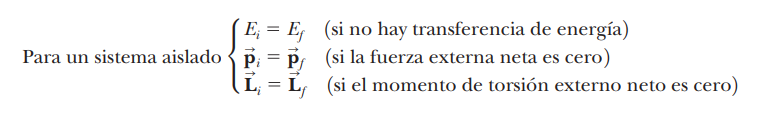
\includegraphics[width = 275px]{conservacion.png}\\

\begin{equation*}
	E = \frac{1}{2}k A^2
\end{equation*}

\begin{equation}
	T = \dfrac{2\pi}{\omega} = 2\pi \sqrt{\dfrac{L}{g}}
\end{equation}


\end{document}